\title {Controlling vergence with \\ an antrophomorphic head}
\author{Francesco Nori}
\date{$16^{th}$ November 2006}
\maketitle

\begin{abstract}
In this report we discuss the implementation of a vergence controller on a humanoid robot. Specific attention will be posed on controlling the two eyes so as to verge on the hand. Experiments with our humanoid robot James will be discussed. The problem of creating a realistic model of the hand is a stand alone problem which falls outside the scope of this project. Therefore in the present experiments, the hand localization problem will be simplified by attaching a marker to the hand. Future experiments will be based on a self-constructed model of the hand.
\end{abstract}

\section{The system description}

\begin{figure}[h!tbp]
\centering
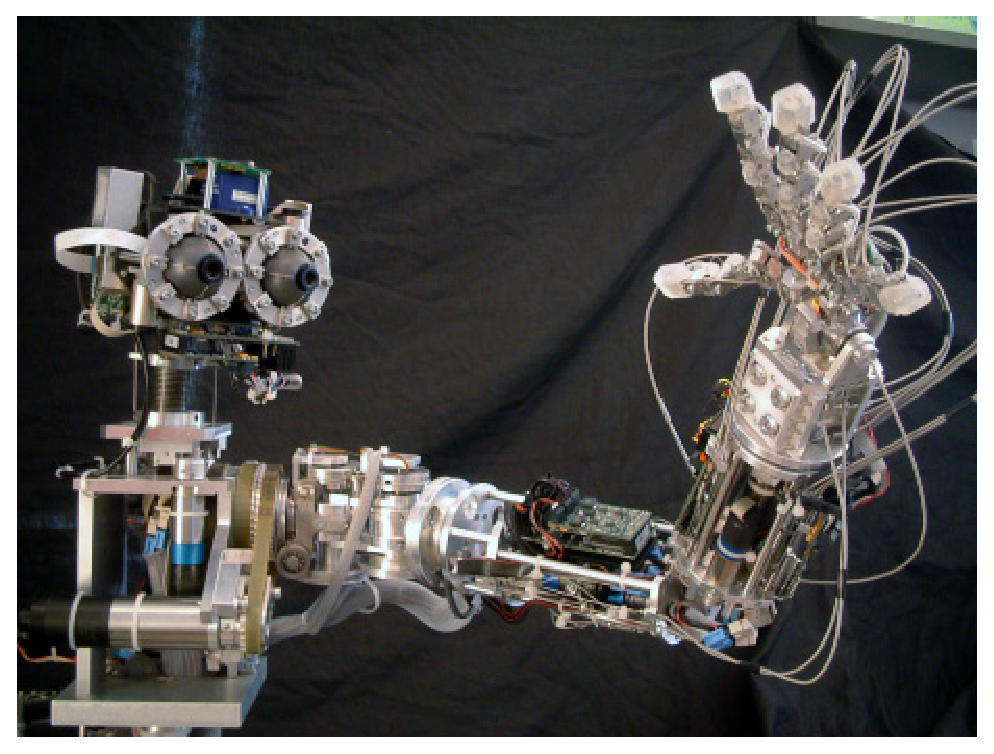
\includegraphics[width=80mm]{Figure/James1.eps}
\caption{The humanoid robot James.}
\label{Fig:PictureJames}
\end{figure}

The fixation controller has been implemented on our humanoid robot James (see figure \ref{Fig:PictureJames}). James consists of 22 DOFs, actuated by a total of 23 motors, whose torque is transmitted to the joints by belts and stainless-steel tendons. The head is equipped with two eyes, which can pan and tilt independently (4 DOFs), and is mounted on a 3-DOF neck, which allows the movement of the head as needed in the 3D rotational space.


\subsection{Head-eye actuation structure}

\begin{figure}[h!tbp]
  % Requires \usepackage{graphicx}
  \centering
  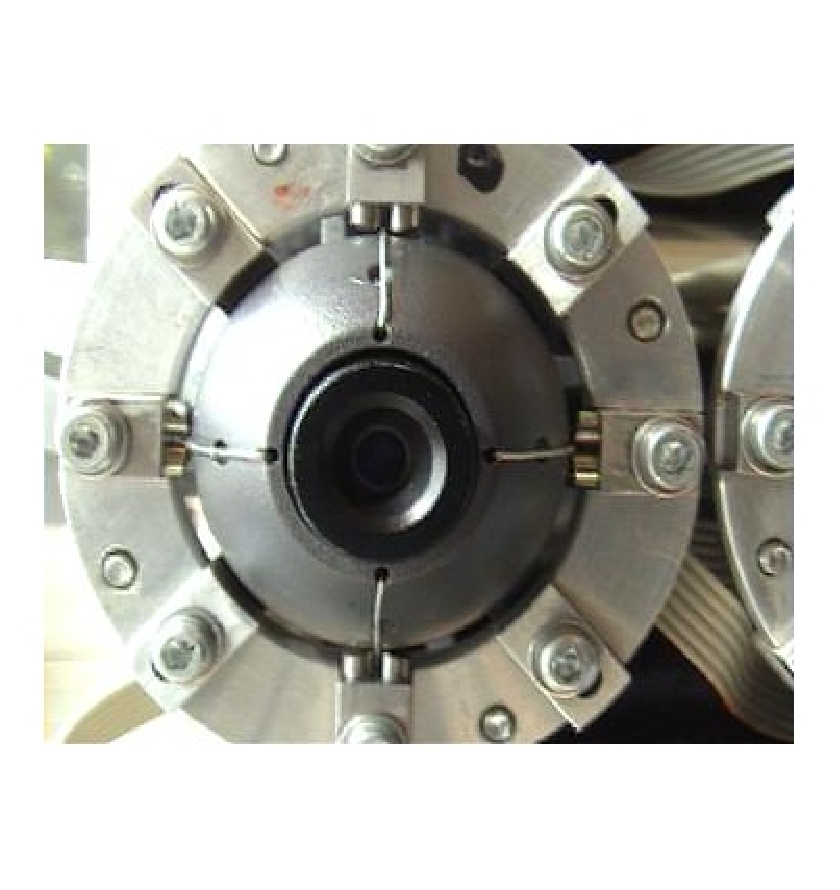
\includegraphics[width=60mm]{Figure/EyePhoto.eps}
  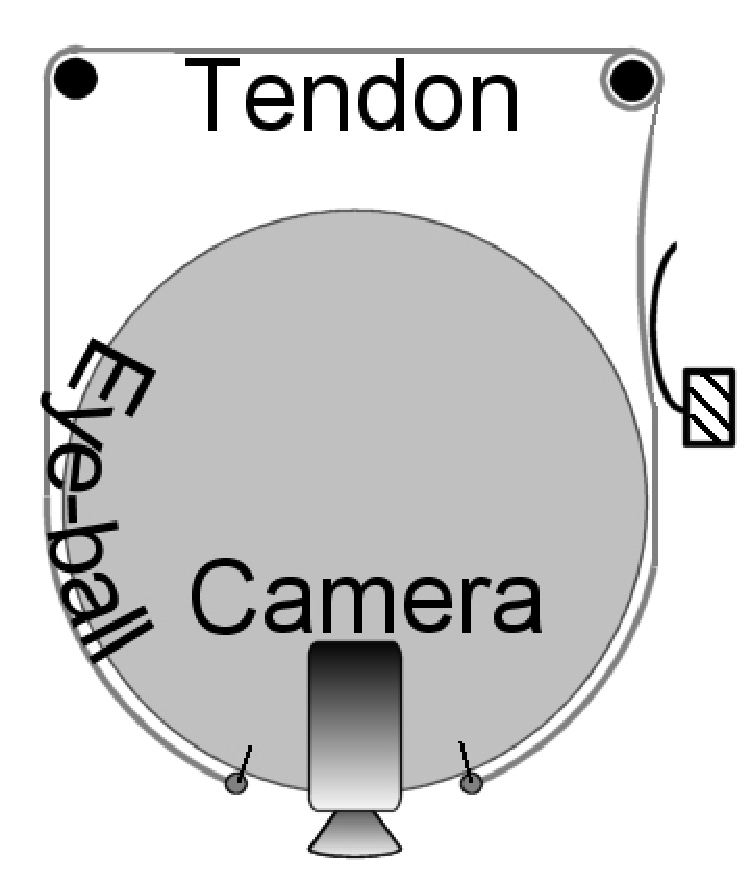
\includegraphics[width=60mm]{Figure/EyeSection.eps}\\
  \caption{The left picture shows the tendon driven eye. The
 two tendons are actuated by two motors. The first motor moves the vertical
  tendon (tilt motion). The second motor moves the horizontal tendon (pan motion). The
  right figure sketches the actuation scheme.}\label{Fig:EyeSection}
\end{figure}

The head structure has a total of 7 degrees of freedom, actuated by 8 motors. Four of these motors are used to actuate the pan and tilt movements of the two independent eyes (see Figure \ref{Fig:EyeSection} for a scheme of the tendon actuation). One motor directly actuates the head yaw. The remaining three motors actuate the head's two additional rotations: pithc and roll. These two rotations are achieved with an unconventional actuation system (see Figure \ref{Fig:Head}). Each motor pulls a tendon; the tension of the three tendons determines the equilibrium configuration of the spring on which the head is mounted. The structure has an implicit compliance but it can become fairly stiff when needed by pulling the three tendons simultaneously.

\begin{figure}[tbp]
\centering
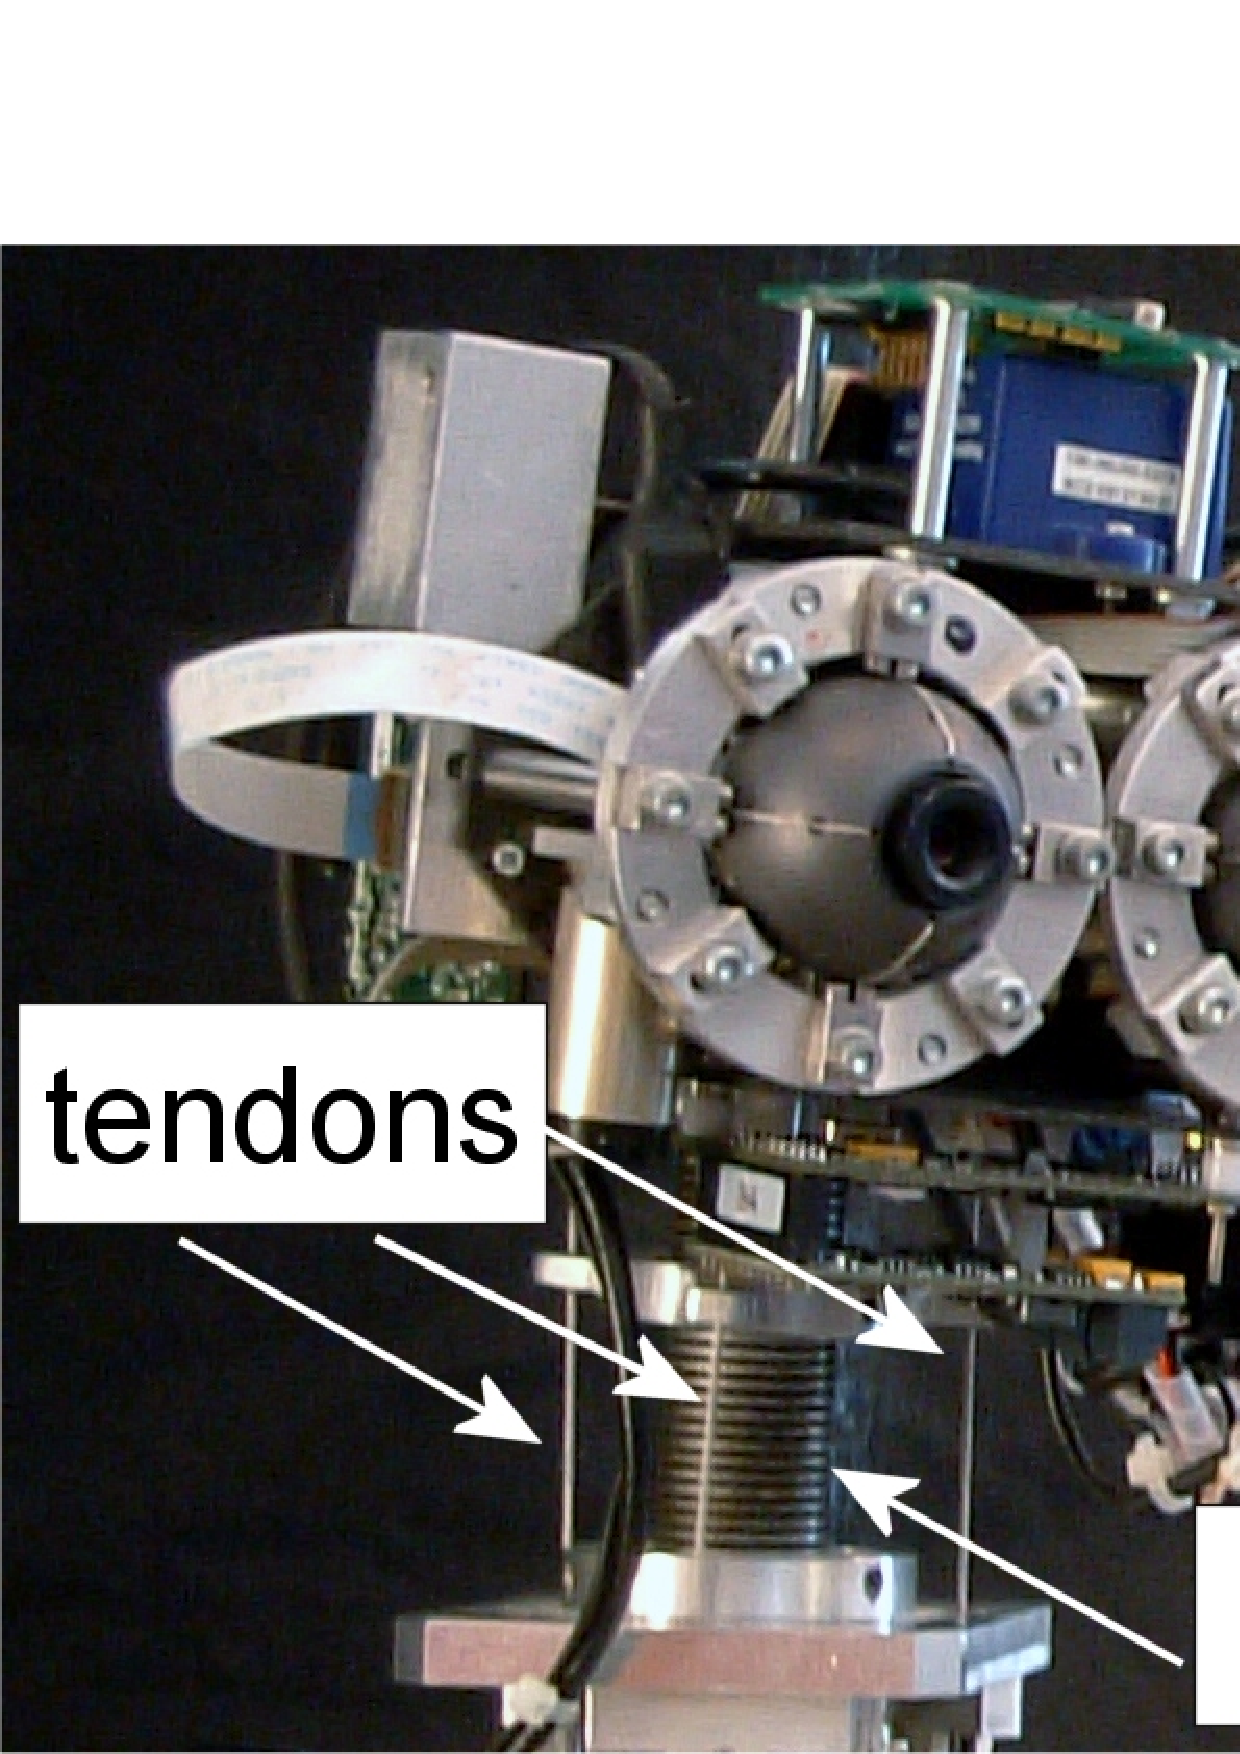
\includegraphics[width=80mm]{Figure/Head.jpg}
\caption{The pictures describes the neck actuation. Practically, the head is mounted on a spring. The spring is moved by pushing and pulling three tendons by the use of conventional DC motors.}
\label{Fig:Head}
\end{figure}

\section{Control of the neck}

The neck is characterized by an original structure and has required the design of an original control technique. The final design is based on the use of an inertia sensor, which has been positioned on the top of the robot head. The sensor measures the (absolute) rotation\footnote{The rotation is expressed by three angles which will be denoted roll ($\theta_r$), pitch ($\theta_p$) and yaw ($\theta_y$). The three motors of the neck influence the first two angles ($\theta_r$), pitch ($\theta_p$). The remaining degree of rotation ($\theta_y$) is directly influenced by the head pan which is moved by a specific motor.} of the head with respect to an inertial reference frame. Using the information from this sensor we developed a closed loop controller to position the head in any desired configuration. 

\subsection{Neck control in details}

The development of the control loop has required the development of a \textsc{Matlab} model of the neck structure. The model is based on the assumption that the spring has a constant length (since it is always compressed). When the spring is bended, the assumption is that its curvature is constant along the entire spring length. Using this model we were able to compute the ideal tendons lengths given the pose of the neck, or equivalently the ideal tendons lengths ($l_1$, $l_2$, $l_3$) given the inertia sensor measurement ($\theta_r$, $\theta_p$). Practically, the model of the system is a function $f: \mathbb R^3 \longrightarrow \mathbb R^3$ such that:
\begin{eqnarray} \label{Eq:Model}
\begin{bmatrix}
l_1\\
l_2\\
l_3
\end{bmatrix} = f (\theta_r, \theta_p).
\end{eqnarray}

The final control loop for positioning the neck in the desired configuration ($\theta_r^d$, $\theta_p^d$) is the following:
\begin{eqnarray} \label{Eq:Control_V1}
\begin{bmatrix}
\frac{d l_1}{dt}\\
\frac{d l_2}{dt}\\
\frac{d l_3}{dt}
\end{bmatrix} = -\begin{bmatrix} \frac{\partial f} {\partial \theta_r} &  \frac{\partial f} {\partial \theta_p} \end{bmatrix}
 \begin{bmatrix}
\theta_r - \theta_r^d\\
\theta_p - \theta_p^d
\end{bmatrix},
\end{eqnarray}
where $\begin{bmatrix} \frac{\partial f} {\partial \theta_r} &  \frac{\partial f} {\partial \theta_p} \end{bmatrix}$ is the Jacobian of the function $f$ with respect to $\theta_r$, $\theta_p$ computed at the current configuration $\theta_r$, $\theta_p$. 

The above model (\ref{Eq:Model}) is ideal and assumes that the three tendons are always stretched. Practically, it is always desirable to have the stretched tendons. However, due to the imperfections in the model, the tendons may loose tension if the control strategy (\ref{Eq:Control_V1}) is applied for a long time. The final solution has been to apply a different control strategy which mixes two different controllers:
\begin{eqnarray} \label{Eq:Control_V2}
\begin{bmatrix}
\frac{d l_1}{dt}\\
\frac{d l_2}{dt}\\
\frac{d l_3}{dt}
\end{bmatrix} = -(1-\gamma)\begin{bmatrix} \frac{\partial f} {\partial \theta_r} &  \frac{\partial f} {\partial \theta_p} \end{bmatrix}
 \begin{bmatrix}
\theta_r - \theta_r^d\\
\theta_p - \theta_p^d
\end{bmatrix} - \gamma \left( \begin{bmatrix} l_1\\
l_2\\
l_3
\end{bmatrix} - f(\theta_r, \theta_p) \right),
\end{eqnarray}
where $\gamma$ is an arbitrary value in the interval $[0, 1]$. The second term of the controller (the one multiplied by $\gamma$) guarantees that the the length of the cables remains similar to the length of the model. This strategy is sufficient to guarantee that the tendons maintain a tension which is more or less constant among the different configurations. In this final configuration the jacobian $\begin{bmatrix} \frac{\partial f} {\partial \theta_r} &  \frac{\partial f} {\partial \theta_p} \end{bmatrix}$ can be substituted with a constant jacobian computed at the reference configuration $\theta_r$=$\theta_p$=0.

\section{Vergence controller}

\begin{figure}[tbp]
\centering
\includegraphics[width=120mm]{Figure/SteroImages.jpg}
\caption{Two typical images taken from the two cameras mounted on the eyes of the robot. The attention system gives us the target position on the two image planes. The coordinates of the target on the right image plane will be denoted $u_r$, $v_r$, while on the left image will be denoted $u_l$, $v_l$. The vergence controller task is to move the eyes and the neck in order to keep the target point at the center of the two image planes, i.e. $u_r = v_r = u_l = v_l = 0$.}
\label{Fig:ImagePlane}
\end{figure}

We implemented a control strategy for verging on a target (blue ball) which has been attached to the robot hand. We assume that there's an attention system on the robot capable of localizing the target on the image plane. Let $u_r$ and $v_r$ be the coordinates of the target on the right image plane. Similarly, let $u_l$ and $v_l$ be the coordinates of the target on the left image plane. 

The strategy we have chosen consists in using a dominant eye (in our case the left eye) to perform a saccade on the desired target and then to follow the dominant eye movement with the neck. This choice is a consequence of the fact that the eyes can make fast movement because of their low inertia. However, their range of movement is small if compared with the neck movement which is characterized by a pretty big range even if with a bigger inertia. This strategy allows us to keep the target always at the center of the image while also allowing a big range of movement for the target itself. Mathematically the above strategy can be implemented as follows:

\begin{eqnarray} 
\left\{ \begin{matrix}
\frac{d \alpha_p^l}{ d t} &=&   K_p u_l\\
\frac{d \theta_y}{ d t} &=&   K_y \alpha_p^l \\
\frac{d \alpha_t^l} {d t} &=&   K_t v_l\\
\frac{d \theta_p} {d t} &=&   K_r \alpha_t^l
\end{matrix} \right.,
\end{eqnarray}
where $\alpha_p^l$ and $\alpha_t^l$ are the pan and tilt positions of the left eye and where $\theta_y$ and $\theta_p$ are the yaw and pitch movement of the neck. This control strategy allows us to asymptotically fixate the target with the left eye ($u_l \rightarrow 0$, $v_l \rightarrow 0$) while also also guaranteeing an asymptotically  straight gaze ($\alpha_p^l \rightarrow 0$, $\alpha_t^l \rightarrow 0$). Another possible control strategy which takes into account the fact that the eye movements anticipate the neck movements is the following:
\begin{eqnarray} \label{Eq:HeadEyeControl}
\left\{ \begin{matrix}
\frac{d \alpha_p^l}{ d t} &=&   K_p u_l\\
\frac{d \theta_y}{ d t} &=&   K_y \alpha_p^l + K_{yp} u_l\\
\frac{d \alpha_t^l} {d t} &=&   K_t v_l\\
\frac{d \theta_p} {d t} &=&   K_r \alpha_t^l + K_{yt} v_l
\end{matrix} \right. .
\end{eqnarray}
In order to verge on the target (i.e. $u_l \rightarrow 0$, $v_l \rightarrow 0$, $u_r \rightarrow 0$, $v_r \rightarrow 0$), we need also to guarantee that $u_r \rightarrow 0$ and $v_r \rightarrow 0$. Assuming that the two cameras are aligned (up to a calibration of the system), we have that $v_r \rightarrow 0$ is automatically implied by $v_l \rightarrow 0$. We are therefore left with guaranteeing that $u_r \rightarrow 0$. This is trivially guaranteed by the following control law:
\begin{eqnarray} \label{Eq:EyeVergenceControl}
\frac{d \alpha_p^r}{ d t} &=&   K_p u_r
\end{eqnarray}
Using the above control strategy (\ref{Eq:HeadEyeControl}) and (\ref{Eq:EyeVergenceControl}),  we obtained the tracking results shown in Figure \ref{Fig:TimeResponse}.

\begin{figure}[tbp]
\centering
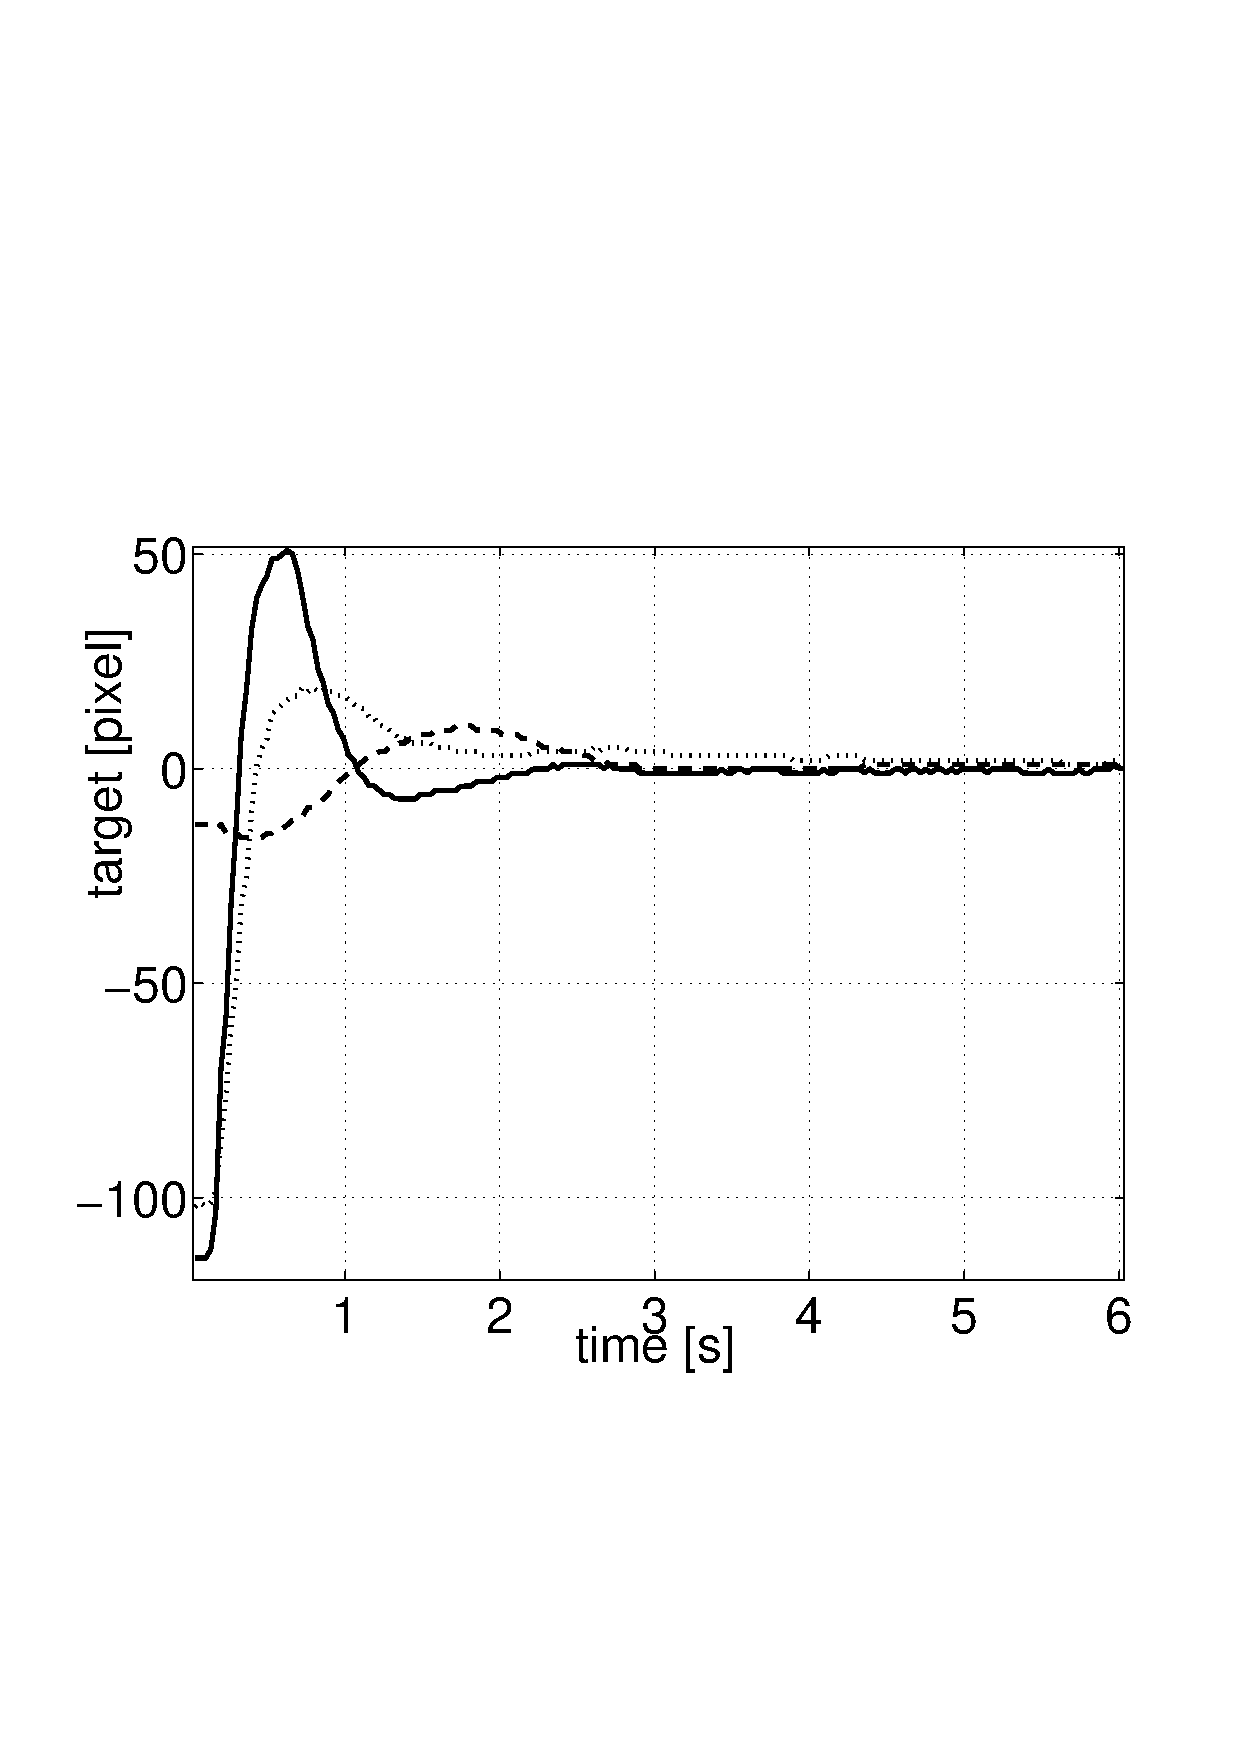
\includegraphics[width=130mm]{Figure/TimeResponseImage.jpg}
\caption{The picture shows the time response of the tracking behavior of the fixation controller. The picture shows that the target is effectively driven to the image center (up to an accuracy of one pixel).}
\label{Fig:TimeResponse}
\end{figure}

\begin{figure}[tbp]
\centering
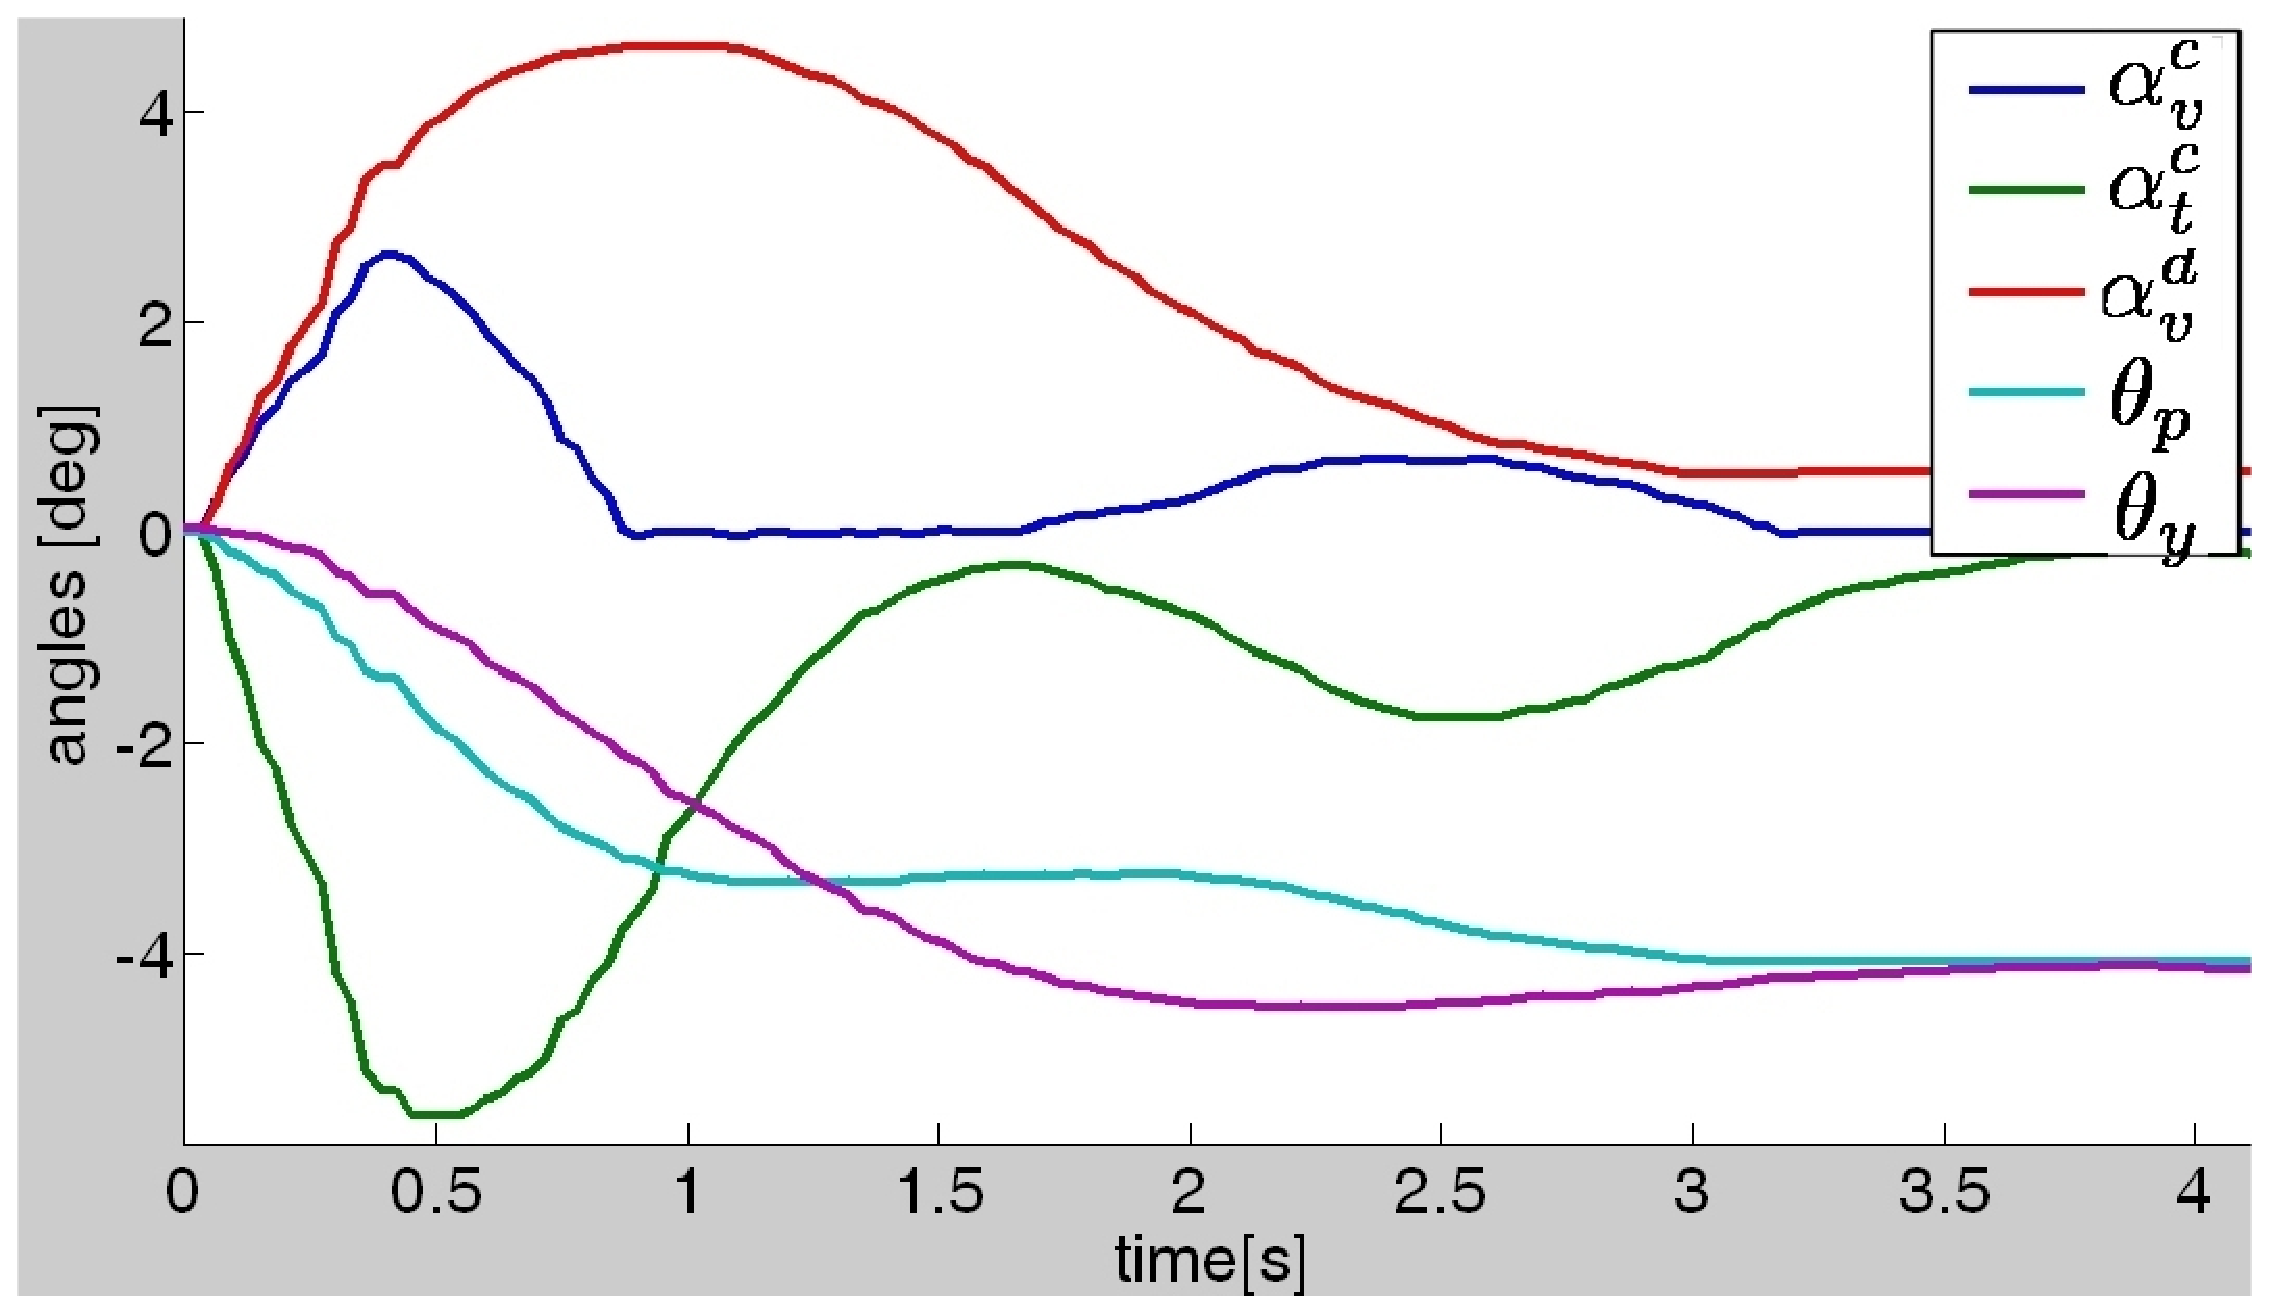
\includegraphics[width=130mm]{Figure/TimeResponseEyesNeck.eps}
\caption{The picture shows the time response of the tracking behavior of the fixation controller. The picture shows that the dominant eye (left eye) is effectively driven to straight gaze configuration ($\alpha_p^l \rightarrow 0$, $\alpha_t^l \rightarrow 0$ up to an accuracy of one degree). The neck is instead positioned so as to face the target.}
\label{Fig:TimeResponseNeck}
\end{figure}
